\documentclass{article}
\usepackage[a4paper, margin=.5in]{geometry}
\usepackage{amssymb}
\usepackage{parskip}
\usepackage{graphicx}
\graphicspath{ {./images/} }
\title{Unit 3 Test Cheatsheet}
\date{}
\begin{document}
\maketitle
\textbf{1.1 Set Theory:}\\
Union: $A \cup B = \{x \mid x \in A \lor x \in B\}$; Intersection: $A \cap B = \{x \mid x \in A \land x \in B\}$\\
$A$ and $B$ are disjoint: $A \cap B = \varnothing$\\
Difference: $A - B = \{x \mid x \in A \land x \notin B\}$\\
Distribution: $A \cap (B \cup C) = (A \cap B) \cup (A \cap C)$; $A \cup (B \cap C) = (A \cup B) \cap (A \cup C)$\\
DeMorgan: $A - (B \cup C) = (A - B) \cap (A - C)$; $A - (B \cap C) = (A - B) \cup (A - C)$\\
Power set of A: $\mathcal{P}(A)$ is the set of all subsets of $A$ (including $A$ and $\varnothing$)\\\
Arbitrary union: $\bigcup_{A \in \mathcal{A}} A = \{x \mid x \in A$ for at least one $A \in \mathcal{A}\}$ (where $\mathcal{A}$ is a collection of sets)\\
Arbitrary intersection: $\bigcap_{A \in \mathcal{A}} A = \{x \mid x \in A$ for every $A \in \mathcal{A}\}$ (undefined when $\mathcal{A} = \varnothing$)\\
Cartesian product: $A \times B = \{(a, b) \mid a \in A \land b \in B\}$ (set of all ordered pairs $(a, b)$ where $a \in A$ and $b \in B$)\\

\textbf{1.2 Functions:}\\
Rule of assignment: subset $r$ of the Cartesian product $C \times D$ of two sets, having the property that each element of $C$ appears as the first coordinate of at most one ordered pair in $r$ (i.e. every thing in the domain is mapped to no more than one thing in the range)
\begin{itemize}
    \item $r$ is a rule of assignment if $(c, d) \in r \land (c, d') \in r \Rightarrow d=d'$
    \item Domain: subset of $C$ consisting of all first coordinates of $r$; $\{c \mid$ there exists $d\in D$ such that $(c, d) \in r\}$
    \item Image: subset of $C$ consisting of all second coordinates of $r$ (everything that actually gets mapped to); \\$\{d \mid$ there exists $c\in C$ such that $(c, d) \in r\}$
\end{itemize}
Function $f$: rule of assignment $r$ with a set $B$ that contains the image set of $r$. The domain $A$ of $r$ is also the domain of $f$; image set of $r$ is the image set of $f$; $B$ is the range of $f$.
\begin{itemize}
    \item $f(a)$ is the unique element of $B$ such that $(a, f(a)) \in r$
    \item Let $A_{0} \subset A$. Restriction of $f$ to $A_{0}$: $\{(a, f(a)) \mid a \in A_{0}\}$
    \item Image of $A_{0}$ under $f$: $f(A_{0}) = \{b \mid b = f(a)$ for at least one $a \in A_{0}\}$
    \item Changing the domain or range changes the function
\end{itemize}
Composition of functions: given $f:A \to B$ and $g:B \to C$, $g \circ f:A \to C$ is defined by $g \circ f (a) = g(f(a))$ 
\begin{itemize}
    \item Only defined when the range of $f$ equals the domain of $g$
    \item Alternately: $g \circ f : A \to C = \{(a, c) \mid$ For some $b \in B, f(a) = b \land g(b) = c\}$
\end{itemize}
Injective: no two distinct points in the domain map to the same point in the range; every point in the range is mapped to by at most one point in the domain; $f(a) = f(a') \Rightarrow a = a'$\\
Surjective: every point in the range is mapped to; $b \in B \Rightarrow (b = f(a)$ for at least one $a \in A)$\\
Inverse: exists if $f$ is bijective; $f^{-1}(B_{0}) = \{a \mid f(a) \in B_{0}\}$\\

\textbf{1.3 Relations:}\\
Relation: a relation on $A$ is a subset $C$ of $A \times A$\\
Equivalence relation has 3 properties:
\begin{itemize}
    \item Reflexivity: $xCx$ for every $x \in A$
    \item Symmetry: If $xCy$, then $yCx$
    \item Transitivity: If $xCy$ and $yCz$, then $xCz$
\end{itemize}
Equivalence class determined by x: $\{y \mid y \sim x\}$
\begin{itemize}
    \item Always contains $x$
    \item Two equivalence classes $E$ and $E'$ are either disjoint or equal\\ 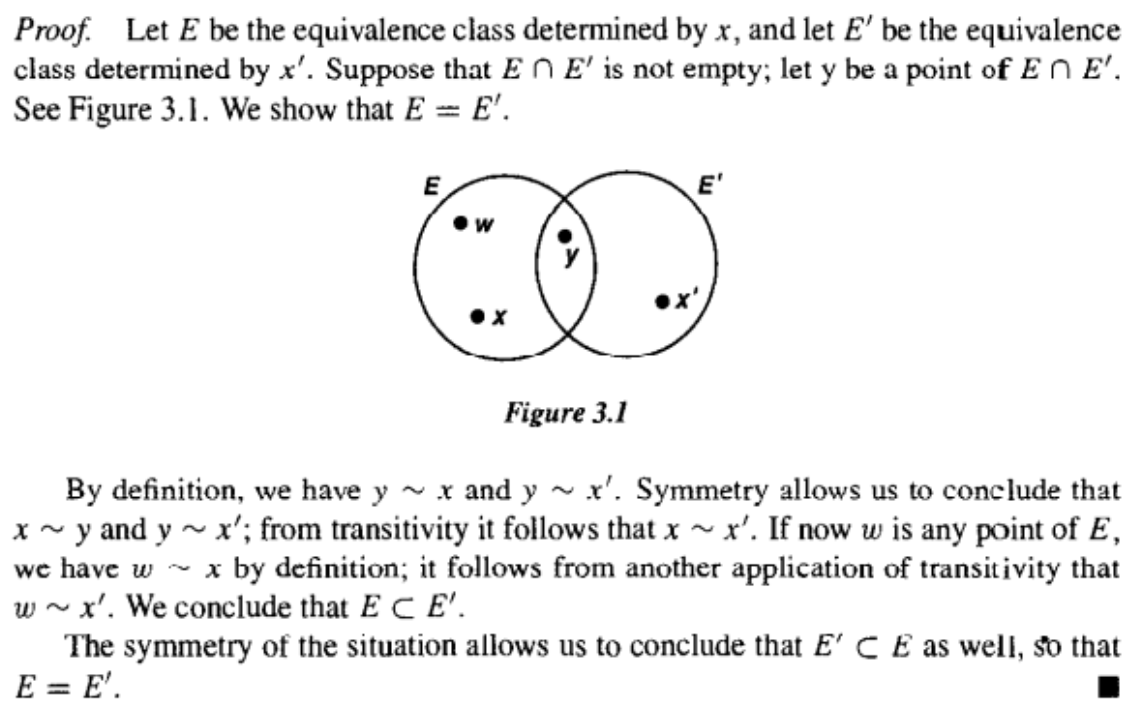
\includegraphics[scale=0.6]{test3StudyProofEquivalenceClasses.png}
\end{itemize}
Partition of set A: collection of disjoint, nonempty sets of $A$, where the union of these sets is all of $A$; any partition of $A$ comes from exactly one equivalence relation on $A$\\
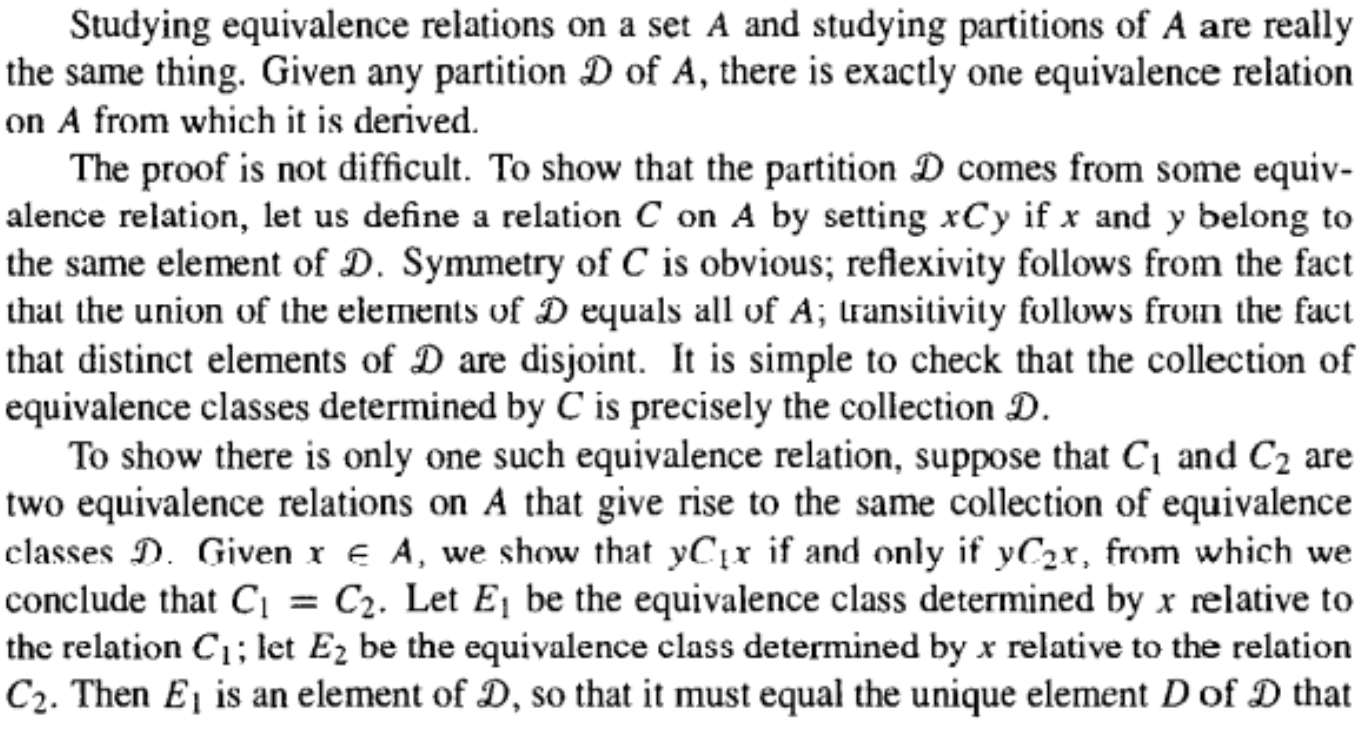
\includegraphics[scale=0.75]{test3StudyProofPartitions1.png}\\
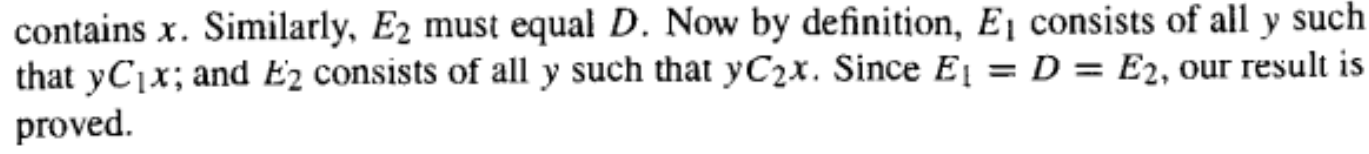
\includegraphics[scale=0.75]{test3StudyProofPartitions2.png}\\
\end{document}
